\section{Algorithms and Proofs}
\label{choiceOfMethod}

\subsection{Introduction}
In this section I will describe the two main algorithms I have used in this project and discuss their merits and flaws. At the end of this section I will also give several proofs that I need i this project.

\subsection{Possible Methods}

\begin{description}
\item[Computational Geometry:] The intuitive description of the Lonely Runner conjecture (\nref{introduction}) lends itself well to a geometrical interpretation, and leads me to wonder whether such an algorithm could efficiently find a solution.

\item[Numerical:] The Lonely Runner conjecture is, in its original formulation, a problem from number theory. It is therefore reasonable to assume that a Numerical approach would lead to an efficient algorithm.
\end{description}

\subsection{Computational Geometry}
\label{compGeo}
The following solution is one of my own devising, based on the first intuitive description of the conjecture found in Section \ref{introduction}. It is clear that we are interested in the time interval when the runners are in the Zone, but not where in the Zone the individual runners are. We are thus only interested when a runner enters and leaves the Zone. 

Let $s$ be the speed of a given runner then the runner enters the Zone for the first time when he is $\frac{1}{n+1}$ units away from the start line, and leaves it when he has passed $\frac{n}{n+1}$ units.
Therefore the runner first enters the Zone at: 

\begin{equation}
\label{eqa:speedOne}
\begin{split}
s * t &= \frac{1}{n+1} \\
t &= \frac{1}{s * (n+1)}
\end{split}
\end{equation}

and leaves the Zone at time:

\begin{equation}
\label{eqa:speedTwo}
\begin{split}
s * t &= \frac{n}{n+1} \\
t &= \frac{n}{s * (n+1)}
\end{split}
\end{equation}

From \eqaref{eqa:speedOne} and \eqaref{eqa:speedTwo} it is clear that the time interval for the first time the runner is in the Zone will be 
\begin{displaymath}
\left[\frac{1}{s * (n+1)}, \frac{n}{s * (n+1)}\right]
\end{displaymath}

More generally, a runner with speed $s$ will be in the Zone for the $k$'th time, where $k \in \N \cup \E{0}$, in the time interval 

\begin{equation}
\label{eqa:genericZone}
\left[\frac{1 + k * (n+1)}{s * (n+1)}, \frac{n + k * (n+1)}{s * (n+1)}\right] 
\end{equation}

So in order to find a time where all the runners are in the Zone (which would make \eqaref{eqa:lonelyRunner} hold), we need to check whether or not there is a time that is contained in the intervals produced by the runners. To do this I propose using a horizontal Plane Sweep algorithm\footnote{For a general overview of Plane Sweep algorithms, please consult \cite{citeulike:3347056} or any other university level, or higher textbook dealing with Computational Geometry}, where the interesting cases are when a runner enters and leaves the Zone. 

\subsubsection{High Level Description of the Algorithm}

\begin{algorithm}[H]
  \caption{SimpleLonelyRunner\label{simpleLonelyRunner}}
  \highlights
  \SetKwData{and}{and}
  \Input{A list \s which contains $n$ pairwise different speeds for $n$ runners}
  \Output{A time \ti where all $n$ runners are at least $\frac{1}{n + 1}$ units away from the starting line, or a \no, indicating that no such time exists}
  
  Make \finish with time $1$ and add it to \li

  \ForEach{speed $\in$ \s}{
    
    Make the first \startT and \eT based on speed - see \eqaref{eqa:speedOne} and \eqaref{eqa:speedTwo}, and insert it in \li
  }
  
  \While{\true}{

    Pop Event Point \p from \li
    
    \If{\p is \startT}{      
      
      Record that a runner has entered the Zone

      \If{all the runners are in the Zone}{
        \return $\p_{\ti}$
      }
    }
    
    \uElseIf{\p is \eT}{
      
      Record that a runner has left the Zone

      Make the next \startT and \eT based on \eT and add them to \li
    }
    \ElseIf{\p is \finish}{
      \return \no
    }
  }
\end{algorithm}

See figure \ref{algoIlluImg} for an intuitive illustration of idea behind the algorithm. 

\begin{figure}[H]
  \centering
  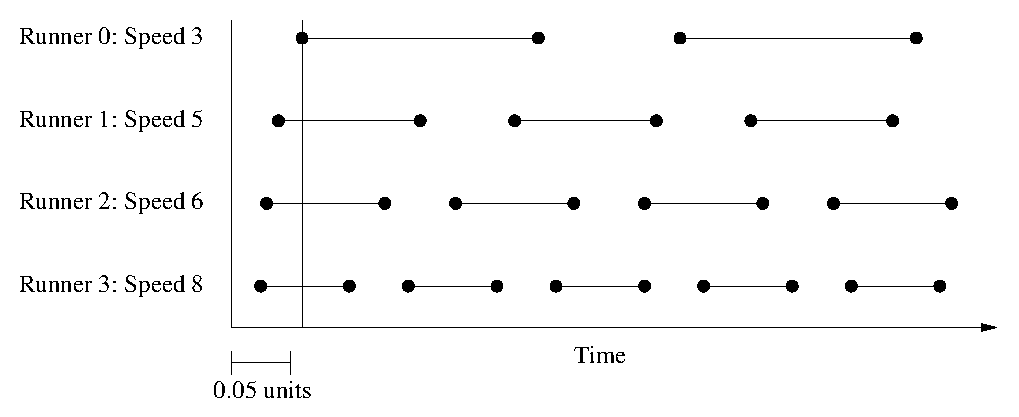
\includegraphics[width=\textwidth]{./images/algoIlluEPS}
  \caption{\label{algoIlluImg}An illustration of the Plane Sweep algorithm with the canonical speeds: 3, 5, 6 and 8. The dots are the Event Points, and the horizontal line between Event Points are when a given runner is in the Zone. The Vertical line is the sweep line, which jumps from Event Point to Event Point from the left to the right, ignoring everything in-between. The vertical line is here placed at the first time where \eqaref{eqa:lonelyRunner} holds for the speeds 3, 5, 6 and 8.}
\end{figure}

\subsubsection{Termination Criteria}
\label{termination}
Since the Lonely Runner conjecture has not been proved for all $n \in \N$, there must be a means to terminate the algorithm, if for a given configuration of runners, there does not exists a time that make \eqaref{eqa:lonelyRunner} hold.

My solution to this is to introduce the fake runner. The fake runner has a speed of $1$, and will only serve as a marker for when to terminate the algorithm. The intuition behind this is that based on \eqaref{eqa:lonelyRunner} - it is clear that if a solution exist it must do so for $x \in \mathbb{T}$, and therefore if we reach the time $1$, no solution to \eqaref{eqa:lonelyRunner} exists.

\begin{lemma}
\label{maximum_event_points}
I will in this lemma prove that given $n$ runners there will be at most $2n + 1$, and therefore at most $O(n)$ Event Points in the Priority Queue:

When the algorithm enters the main loop it is clear from algorithm \ref{simpleLonelyRunner} that there must be $2n + 1$ Event Points in the Priority Queue. We have $1$ point from the fake runner, and $2n$ points from the real runners. In the main loop it is only when an \comEnd has been removed from the Priority Queue that more points can be added, and furthermore it is clear that an \comEnd can only be removed if its \comStart\;has been removed first. Since precisely 2 Event Points are added to the Priority Queue each time we encounter an \comEnd, and at least 2 Event Points have to have been removed for this to happen, the number of Event Points in the Priority Queue can never exceed $2n + 1$, and must therefore at most contain $O(n)$ Event Points, which was what we wanted to show.
\end{lemma}

\subsubsection{Proofs of the Geometric Algorithm}
\label{proof_geo}

\begin{theo}[Correctness:]
The main idea of the algorithm is that it keeps track when runners enters and leaves the Zone, and iff it finds that all runners are in the Zone, then it reports the solution. The only way the algorithm can fail is therefore if either

\begin{description}
\item[Case A:] If a runner can enter the at time $t_{enter}$ Zone without the distance to the start line being $\frac{1}{n+1}$ units. 
\item[Case B:] If a runner can leave the at time $t_{leave}$ Zone without the shortest distance to the start line being $\frac{1}{n+1}$ units.  
\end{description}
Let $dist_r$(t): $\R \rightarrow \mathbb{T}$ be the distance function from the start line in the runners direction to the runner r at time t along the circular track.

Let entering the Zone at time $t_{enter}$ mean that $dist_r(t_{enter})$ is in the Zone, while $dist_r(t_{prev})$ is not in the Zone, where $t_{prev} = \max\E{x \in \R: x < t_{enter}}$. Analogusly let leaving the Zone at time $t_{leave}$ mean that $dist_r(t_{leave})$ is in the Zone, while $dist_r(t_{next})$ is not in the Zone, where $t_{next} = \min\E{x \in \R: t_{leave} < x}$.
 
I will now prove that neither case A or B can happen, and thus my algorithm will always give the correct result.

\begin{description}
\item[Case A:]I will prove case A cannot happen, by proof by contradiction:
Let us assume that the runner r enters the Zone at time $t_{enter}$, and that $dist_r(t_{enter}) \in (\frac{1}{n+1}, \frac{n}{n+1}]$. As defined above, there must therefore exist a time $t_{prev}$ just before $t_{enter}$ where $dist_r(t_{prev})$ is after the start line, but before the Zone. 

We now have a closed interval $[dist_r(t_{prev}), dist_r(t_{enter})]$, for which the function clearly is continuous, it then follows from the Intermediate value theorem that there must exist a time $t_{real\_enter}$ where $dist_r(t_{real\_enter}) = \frac{1}{n+1}$. This however contradicts our assumption that the runner enters the Zone at $dist_r(t_{enter}) \in (\frac{1}{n+1}, \frac{n}{n+1}]$, and so therefore the runner must always enter the Zone at distance $\frac{1}{n+1}$ from the start line, which means that case A cannot happen, which was what I wanted to show.
\item[Case B:]Case B can be proved analogously, with $dist_r(t_{leave}) \in [\frac{1}{n+1}, \frac{n}{n+1})$, and $dist_r(t_{next})$ not being in the Zone, but before the startline.
\end{description}
Since neither Case A or Case B can happen, the Geometrical algorithm will always report the correct result.
\end{theo}

\begin{theo}[Termination:]
It is clear that the algorithm will always terminate, since the algorithm terminates when it finds a timepoint where all the runners are in the Zone, or when it encounters \comFin\,(which cannot be removed prematurely).
\end{theo}

\begin{theo}[Time complexity:]
The first loop of the algorithm takes $O(n\log(n))$ time, since it has to add $2n$ Event Points to the Priority Queue, where each insertion taking $O(\log(n))$.\\

After the first loop, there will at most be $2n + 1$ or $O(n)$ Event Points in the Priority Queue, since each time we encounter a \comEnd, two new Event Points are added to the Priority Queue.\\ 

It is clear that the second loop is dependent on how many Event Points are processed before \comFin, at time $1$ is encountered. For any given runner with speed $s$, it is clear that it will make $s$ rounds before the fake runner arrives at the finishing line, and each time  a runner makes a complete tour of the track, the algorithm has to deal with 2 Event Points --- a \comStart\; and an \comEnd. The \comStart\; event takes $O(1)$ to process, while the \comEnd\; will take $O(\log(n))$ time, because of Lemma \ref{maximum_event_points}. Therefore it is clear that if we let  $k$ be the sum of all the runner's speeds, then the algorithm has a time complexity of $O(k\log(n))$.
\end{theo}

\subsubsection{Event Points}
\label{eventPoints}
In this subsection I will discuss the role of Event Points in the Plane Sweep algorithm, as well as define them. 

As stated in Section \ref{compGeo} we are only interested in whether or not a runner is in the Zone, not his exact position on the track. To take advantage of this I introduce the Event Points, which are used to indicate whether a runner is entering, or leaving, the Zone, ignoring all other time points. 

We must decide whether or not we are going to create all Event Points before entering the main loop\footnote{Since I established in Section \ref{termination} we do not need to look at any Event Points that happen after time 1, and it is clear that we can create all the Event Points before entering the main loop.} or if we should create the first pair for each runner, and then generate more Event Points as it becomes necessary. This also has implications whether a Linked-List or a heap, should be used for the Priority Queue that will contain the Event Points. 

\adDis{
Creating all the Event Points in parallel before entering the main loop
}{
\item We can create each runner Event Points in parallel. After the points have been created, the main loop could be run without having to dedicate any resources to creating new events.

\item It would also make the Priority Queue simpler, since instead of a heap, we could simply use a Linked List structure. 
}{
\item Since all the points are generated at the beginning, this would sharply increase the memory footprint of the algorithm.

\item While the Event Points themselves could be generated in parallel, the Priority Queue would serve as a bottleneck. Even if insertion could be done while the other Event Points were still being generated, it would slow down the procedure enormously. The Priority Queue would also have to be sorted, which would take $O(k\log(k))$ time, where $k$ is the sum of all the runners speeds.

\item It would make the program much more complicated
}{
Given that generating an Event Point is a trivial operation, this does not seem like a good idea.
}

\adDis{
Creating event points on the fly
}{
\item We would have a very small memory footprint.
}{
\item Creating every Event Point sequentially could potentially take a lot more time than the parallel solution, but only if the solution lies very close to time 1, in which case it would take a long time anyway.
}{
Creating the Event Points when needed is far simpler than making all the points before the algorithm starts, although it is potentially slower in situations where the solution to \eqaref{eqa:lonelyRunner} is close to $1$ or no solution to the equation exists for the given configuration of runners. 
}

Based on the above I would argue that creating the Event Points when needed is the preferred solution. 

Another important decision we have to make, is to decide how we are going to represent for the time for the Event Points. From \eqaref{eqa:genericZone}, it is clear that the Event Points are going to have times that have rational numbers. Based on the computer specifications in Section \ref{specs}, it would be preferable if we could avoid floating point calculating altogether, instead work with integers.

Since the point of the time property of an Event Point is to compare it with the time of another Event Point, we could try to make this on integer comparisons: Let $n \in \N$ be the number of runners, and $r$ be the runner in question, $a_r \in \E{1, n}$ be the local position within the Zone, let $k_r \in \N$ be the number of rounds runner $r$ has taken, and let $s_r \in \N$ be the speed of runner $r$, then if we are to compare Event Point i's to Event Point j's time, we have from \eqaref{eqa:genericZone}:
  
\begin{equation}
\label{eqa:integerTime}
\begin{split}
\frac{a_i + k_i * (n+1)}{s_i (n+1)} &< \frac{a_j + k_j * (n+1)}{s_j (n+1)} \Leftrightarrow\\
\frac{a_i + k_i * (n+1)}{s_i} &< \frac{a_j + k_j * (n+1)}{s_j} \Leftrightarrow\\
(a_i + k_i * (n+1)) * s_j &< (a_j + k_j * (n+1)) * s_i \Leftrightarrow
\end{split}
\end{equation}

Thus each Event Point must record its local position $a$, the number of rounds $k$ the runner has made, and the runners speed $s$. Besides that, each Event Point should have a runner number, so that all forms of ambiguity can be removed (see \ref{order}).

In order to distinguish entering and leaving the Zone, and the fake runner I introduce 3 different types of Event Points:
\begin{description}
\item[\comStart] The first point represents the time where the runner is $\frac{1}{n + 1}$ units away from the start line.
\item[\comEnd] The first point after the \comStart\, where the runner is $\frac{1}{n + 1}$ units away from the start line. Since \comEnd\, is the last Event Point for any given runner in the Priority Queue, \comEnd\, will be used to signal that the algorithm must add new a \comStart\, and \comEnd\ to the Priority Queue.
\item[\comFin] The final point in that will be processed --- which has set values of $a = n+1$, $k = 1$ and $s = 1$ and runner number to $n+1$. If this point is ever reached, then \eqaref{eqa:lonelyRunner} does not hold for the given configuration - and the configuration would serve as a counterexample to the Lonely Runner conjecture.
\end{description}

\subsubsection{Order of Points}
\label{order}
In order to avoid any ambiguity concerning the order of the points, I will now define an order $\prec$. \hide{One of the degenerate cases we need to avoid is when we have $(n-1)$ runners that are in the Zone, and the next two points are a \comEnd\, and a \comStart, both at the same time. Since the Zone is a closed set, it is clear that this instance should return a valid solution, but if \comEnd\, comes first, then the solution would not be reported - therefore \comStart\, must be placed before \comEnd.}

\begin{defi}[Order of points]
For the Event Points $p$ and $q$, $p \prec q$ iff
\begin{center}
\label{orderOfPoints}
$p_{time} < q_{time}$\\
or \\
$p_{time} = q_{time}$ and type($q$) = \comFin\\
or \\
$p_{time} = q_{time}$ and type($p$) = \comStart and type($q$) = \comEnd \\
or \\
$p_{time} = q_{time}$ and type($p$) = type($q$) and $p_{runner} < q_{runner}$
\end{center}
\end{defi}

\subsubsection{Psudocode for the Geometrical Algorithm}

\begin{algorithm}[H]
\caption{MakeTimePoints}
\highlights
\SetKwData{start}{startTime}
\Input{The old end point \p and the Event Point queue \li}
\Output{The Event Point queue \li, with a new \startT and \eT inserted the runner \run}
 
Make new \startT $start$ from \p with all the same properties as \p, except that $start_{local\_position} = 1$ and $start_{rounds} = \p_{rounds} + 1$
  
Make new \eT $end$ from \p with all the same properties as \p, except that $end_{local\_position} = p_{number\_of\_runners}$ and $end_{rounds} = \p_{rounds} + 1$
    
Add $start$ and $end$ to \li

\return \li
\end{algorithm}

\begin{algorithm}[H]
  \caption{FindLonelyRunnerTime}
  \highlights
  \SetKwData{and}{and}
  \Input{A list \s which contains $n$ pairwise different speeds for $n$ runners}
  \Output{A point \p where all $n$ runners are at least $\frac{1}{n + 1}$ units away from the starting line, or a \no, indicating that no such time exists}

  Create and initialise \li
  
  \inter $\gets 0$
  
  \n $\gets$ size(\s)
  
  $runnerNum \gets 1$
  
  Make the point \finish with the following properties: $\finish_{number\_of\_runners} = \n$, $\finish_{rounds} = 1$, $\finish_{speed} = 1$, $\finish_{\run} = \n + 1$, $\finish_{local\_position} = n + 1$, and add it to \li

  \ForEach{speed $\in$ \s}{
   
    Make the point \p with the following properties: $\finish_{number\_of\_runners} = \n$, $\finish_{rounds} = -1$, $\finish_{speed} = s$, $\finish_{\run} = runnerNum$, $\finish_{local\_position} = 0$

    \li $\gets$ MakeTimePoints(\p, \li)
    
    $runnerNum += 1$
  }
  
  \While{\li is not empty}{

    \p $\gets$ firstPoint(\li)
    
    \If{\p is \startT}{      
      \inter $+= 1$
    
      \If{\inter == \n}{
        \return $\p$
      }
    }
    
    \uElseIf{\p is \eT}{
    
      \inter $-= 1$
            
      \li $\gets$ MakeTimePoints(\p, \li)
    }
    \ElseIf{\p is \finish}{
      \return \no
    }
  }
\end{algorithm}

\subsection{Numerical Algorithm}
\label{numtheory:algo}
A Numerical alternative to the Geometric algorithm can be made by applying the results of \cite{invis}. The algorithm works by testing a number of time points which might give us a solution - a sort of enlightened guess work. I have sketched the algorithm described from \cite{invis} below. \cite{invis} studies the the function 

\subsubsection{Proofs for the Numerical Algorithm}
\label{proof_num}
\begin{theo}[Correctness:]
This algorithm builds on Theorem 6 in \cite{invis}. Theorem 6 says that if we have a finite set of positive integers D = $\E{d_1, d_2, \ldots, d_k}$, then  $\kappa(D) = \sup_{x \in \R}\min_{1\leq i \leq k}\Vert x d_i \Vert$ is achieved for $x_o = a/(d_i + d_j)$ for some $0 \leq i,j \leq k, i \neq j$, and some positive integer a. I will now paraphrase the proof for this from \cite{invis}:

Let us look at the function $f_D(x) = \min_{1 \leq i \leq k}\Vert x d_i \Vert$. Let $x_0$ be the value that maximises $f_D$, where $x_0 \in \mathbb{T}$. Such an $x_0$ must exist since $f_D$ is continuous, and the circle (and hence) $\mathbb{T}$ is compact. Thus we have $\kappa(D) = f_D(x_0) = \min_{1 \leq i \leq k} \Vert x_0 d_i \Vert$. Let $d_j \in D$ be a value that minimises $\kappa(D)$ and $f_D(x_0)$. We now have that $\kappa(D) = \Vert x_0 d_j\Vert$. 
Furthermore, since all the functions we are dealing with are continuous, there must exist a $d_i \in D$, where $j \neq i$, such that $\Vert x_0 d_j \Vert = \Vert x_0 d_i \Vert$. I will prove that this is the case by proof by contradiction:

Let us assume that $x_0$ such that $\kappa(D) = \Vert x_0 d_j \Vert$, for some $d_j \in D$, and that no $d_i$ exist such that $\Vert x_0 d_j \Vert = \Vert x_0 di\Vert$. In that case, we must have that for all $d_m \in D, m \neq j: \Vert x_0 d_m \Vert > \Vert x_0 d_j$, since we explicitly found $d_j$ to be the value that minimizes $f_D(x_0)$. Then, since $f_D$ is continuous, we can take $y = x_0 \pm \epsilon$ for a small value $\epsilon > 0$, and since $d_j$ was the only value that minimised $f_D(x_0)$, and changing the value of $x_0$ by $\epsilon$ will not change that, we can increase value of $f_D$ so that $f_D(y) > f_D(x_0)$. However, this contradicts our initial assumption that $x_0$ maximises $f_D$, and therefore there must exist a $d_i$ such that $\Vert x_0 d_i \Vert = \Vert x_0 d_j \Vert$.  
 
In fact we have the case $\E{x_0 d_j} = 1 - \E{x_0 d_i}$, where $\E{x}$ is the fractional part of x, i.e. the position on the circle. Thus we have 

\begin{equation}
\begin{split}
x_0d_j + x_0d_i &= \lfloor x_0d_j \rfloor + \E{x_0d_j} + \lfloor x_0d_i \rfloor + \E{x_0d_i} \\
               &= \lfloor x_0d_j \rfloor + \lfloor x_0d_i \rfloor + 1 = a
\end{split} 
\end{equation}

which we can rearrange into $x_0 = a / (d_j + d_i)$, which indeed gives us $\kappa(D)$, which was what we wanted to show.
\end{theo}

\cite{invis} then uses this to prove that their Conjecture 5 is equivalent to the Lonely Runner conjecture, and shows how the finding the value of a will solve their conjecture if the Lonely Runner conjecture holds.

In order to make sure that the Numerical algorithm will always terminate, even in the case where the Lonely Runner conjecture does not hold, I have added the last return statement, ensuring that the correct answer will always be reported.

\begin{theo}[Termination:]
It is clear that the algorithm will always terminate, $\Vert x \Vert $ is the only function call in the algorithm, and it will always terminate.
\end{theo}

\begin{theo}[Time complexity:]
It is clear that the meat of NumericalLonelyRunner is 4 nested for-loops. The 2 first loops are dependent on each other, the third is based on the speed for the two runners that have been chosen, and the last loop goes through all the runners.\\

The first 2 loops gives us $\sum_{i=1}^{n-1}\sum_{j=i+1}^{n}1 = n-1 + n-2 + \ldots 2 + 1$, which reduces to $O(n^2)$. The third loop must iterate $k-1$ times, where $k$ is the sum of 2 runner's speed.\\

If we are to give a worst case time, then it is clear $k$ must be the sum of the speed of the two fastest runners - so if we let $speed_1 = max(\comS)$ and $speed_2 = max(\comS \setminus \E{speed_1})$ then $k = speed_1 + speed_2$
And we go through the last loop $n$ times. Thus the entire algorithm runs in $O(k * n^3)$.
\end{theo}

$$
k(D) = \sup_{x \in \R}\min_{1 \leq i \leq k}\Vert x d_i \Vert
$$
where D is a set $\E{d_1, d_2, \ldots, d_k}$ of integers. They arrive at the result that given D, $k(D)$ ``is attained for $x_0 = a /(d_i + d_j)$ for some $i \neq j$ and some positive integer a''. (Theorem 6 on page 66 in \cite{invis}). It is clear that $a < k$, since if $a = k$ then $a/k$ would evaluate to $1$ and then $\Vert \frac{a}{k} d\Vert, d \in D$ would evaluate to 0, and if $a > k$ then for $n \in \N: \Vert\frac{a}{k}\Vert = \Vert\frac{k+n}{k}\Vert = \Vert\frac{n}{k}\Vert$, so there would be no point in doing so.

\subsubsection{Integer Verification}
Since the Lonely Runner conjecture will always have a rational number as a solution\footnote{We can be sure of this thanks to the correctness proofs for both the Geometrical and the Numerical algorithms in Section \ref{proof_geo} and \ref{proof_num} respectively} (if one such exists), it is clear that we only need to do integer comparison when we need to check whether or not a given $a$ and $k$ gives us a valid solution.

As stated in \eqaref{eqa:lonelyRunner}, we have a Lonely Runner iff
\eqa{
\Vert w_i x\Vert \geq \frac{1}{n+1}
} 

The main problem being $\Vert w_i x\Vert$ - however, since we can be sure that the solution will always be rational, we it must be that x can be written on the form $\frac{p}{q}$ for a given $p \in \N\cup\E{0}$ and $q \in \N$. So now we have

\begin{equation}
\label{compareRewriteOne}
\begin{split}
\Vert w_i * \frac{p}{q}\Vert &\geq \frac{1}{n+1}\\
\min(\frac{w_i * p \bmod q}{q}, 1 - \frac{w_i * p \bmod q}{q}) &\geq \frac{1}{n+1}\\
\min(\frac{w_i * p \bmod q}{q}, 1 - \frac{w_i * p \bmod q}{q}) * (n+1) &\geq 1
\end{split}
\end{equation}

Depending on whether $\frac{w_i * p \mod q}{q}$ or 1 - $\frac{w_i * p \mod q}{q}$ is the smallest value, the equation then becomes

\begin{equation}
\label{compareRewriteTwo}
\begin{split}
\frac{w_i * p \bmod q}{q} * (n+1) &\geq 1\\
(w_i * p \bmod q) * (n+1) &\geq q 
\end{split}
\end{equation}

or 

\begin{equation}
\label{compareRewriteThree}
\begin{split}
1 - \frac{w_i * p \bmod q}{q} * (n+1) &\geq 1\\
(q - (w_i * p \bmod q)) * (n+1) &\geq q
\end{split}
\end{equation}

where we pick the case to analyse on account of which of $w_i * (p \bmod q)$ and $q - (w_i * (p \bmod q))$ are the smallest.

\subsection{Psudocode for the Numerical Algorithm}
\begin{algorithm}[H]
  \caption{NumericalLonelyRunner}
  \highlights
  \SetKwData{and}{and}
  \Input{A list \s which contains $n$ pairwise different speeds for $n$ runners}
  \Output{A time \ti such that all $n$ runners are at least $\frac{1}{n + 1}$ units away from the starting line, or a \no, indicating that no such time exists}
  
  $\n \gets size(\s)$

  \For{$i \gets 1$ \KwTo $\n-1$}{
    
    $d \gets \s_i$
 
    \For{$j \gets i + 1$ \KwTo $\n$}{
      
      $d^{\prime} \gets \s_j$

      $k \gets d + d^{\prime}$
      
      \For{$a \leftarrow 1$ \KwTo $k-1$}{
        
        $testValid \gets true$
        
        \ForEach{$s \in \s$}{
          $distance = \min(s * (a \bmod k),k - (s * (a \bmod k))$
          $testValid \gets testValid\; \and\; (distance * (\n + 1)) \geq k$

          \If{!$testValid$} {
            break
            }
          
        }
        
        \If{testValid}{
          
          \return $\frac{a}{k}$
          
        }
      }
    }
  }
  \return \no
\end{algorithm}

Since the algorithm in worst case tries every single combination of
$d$ and $d\prime$, and \cite{invis} describes no way to detect which
values of $d$ and $d\prime$ that may be candidates for a possible
solution. It is therefore clear that the run-time of the Numerical
algorithm must be dependent on the order of the runner speeds in \comS.



\subsection{Conclusion on the Algorithms}

From the above it is clear that neither of the algorithm are better in all cases. The Geometrical algorithm has a better worst case time complexity when we have many runners with low speeds, while the numerical algorithm is better when we have few runners with very high speeds. It is also clear that the numerical algorithm is far easier to implement, relying on no non-standard data structures.

However, since they both are very short, and do not have much in the way of dependencies, I have implemented them both and have compared their run-times with a variety number of runners and speeds.\\

\subsection{Range Test}
As stated in the introduction, one of the goals of this project was to create a program that could test whether there was a speed configurations in a certain range, that had no solution that made \eqaref{eqa:lonelyRunner} hold. I have interpreted ``range of runner speed configurations'' as follows:\\

Given a \comS of $n$ runners with a maximum speed of $m \in \N$, the program should test all possible configurations between such that for $i, j \in \N, i < j: \comS_i < \comS_j$, where $\comS_n \leq m$. Furthermore I believe the range test to be most useful if it went about its search in a through manner, such that the last index in the $\comS$ should only be increased when all the permutations, with it as the largest value, have been tested\footnote{In practice this means index $n$ would only increase when, for a \comS with 10 runners, has tested the configuration $[\comS_n - 9, \comS_n - 8, \ldots, \comS_n - 1, \comS_n]$}. 

It is important to note that even though a range test has been performed with $n$ runners (say, all possible configurations with 20 runners up to a max speed of 40), then this does not verify any configuration that contains fewer runner. Thus there could theoretically be a configuration with fewer runners in the given speed range that was a counter example for the Lonely Runner conjecture. I have done so because I felt the Range Test tool was designed to check for a specific number of runners, and also that checking every possible   . It should however be little problem to change the code to allow it to test ranges of runners. 

\subsection{The Divisor Check}
\label{detect}
From personal communication with my projects advisor I have been informed of a new method, and its proof, to check whether a configuration makes \eqaref{eqa:lonelyRunner} hold. 

Let $n$ be the number of runners, $S = \E{s_1, s_2, \ldots, s_n}$ be the set of runner speeds, and $p \in \E{2, \ldots, n+1}$. If there exist a $p$ such that it does not evenly divide any of the speeds in $S$, then \eqaref{eqa:lonelyRunner} holds for the set of runner speeds $S$. 

The divisor check cannot stand alone however, as there exist configurations that does make \eqaref{eqa:lonelyRunner} hold, but are not validated by the divisor check. A good example of this is the canonical example, with the speeds 3, 5, 6 and 8. We know from \cite{serra_thelonely} that \eqaref{eqa:lonelyRunner} holds when the number of runners is less or equal to 6, so the canonical example must hold for \eqaref{eqa:lonelyRunner}. But the divisor check clearly fails, since all of the speeds in $\E{2, 3, 4, 5}$ can evenly divide at least one speed in the canonical example.


\subsubsection{Proof}
Let $d_i$ be an arbitrary chosen speed in $S$, and $p \in \E{2, \ldots, n+1}$, be a number that does not divide any number in S. It is clear that we can write $d_i$ as
\begin{equation}
\begin{split}
d_i &= \rfloor\frac{d_i}{p}\lfloor * p + (d_i \bmod p) \Leftrightarrow\\
\frac{d_i}{p} &= \rfloor\frac{d_i}{p}\lfloor + \frac{d_i \bmod p}{p}
\end{split}
\end{equation}

It is clear that $\rfloor\frac{d_i}{p}\lfloor$ is an integer, and that we must therefore have that $(\frac{d_i}{p} \bmod 1) = (\frac{d_i \bmod p}{p} \bmod 1)$. Intuitively we can think of this like the runner with speed $d_i$ runs $\rfloor \frac{d_i}{p}\lfloor$ times around the entire track. It is clear that we can ignore these, and concentrate on $\frac{d_i \bmod p}{p}$. 

We know that $d_i \bmod p \neq 0$, since we assumed $p$ did not evenly divide $d_i$, so it must be that $0 < (d_i \bmod p) < 1$. However, since $p \leq n+1$ we must have that $\frac{1}{n+1} \leq \frac{d_i \bmod p}{p} \leq \frac{n}{n+1}$.

Thus, if we pick the time $\frac{1}{p}$, runner $d_i$ must be in the Zone. Since $d_i$ was an arbitrary chosen speed in $S$, it must hold that all the runners must be in the Zone for $\frac{1}{p}$, and thus the configuration $S$ must hold for \eqaref{eqa:lonelyRunner}, which was what we wanted to show.

\subsection{Integer Speeds}
\label{integerSpeeds}
In this section I will prove that my program will only have to work with integer speeds.
Let us assume for a given configuration of runner speeds T there is a non-empty set $S \subset T$ of runner speeds that are not integers. Since we are dealing with the speeds of runners, it is clear that there are 3 cases we have to worry about: 
\begin{itemize}
\item Either all elements in S belong to $\mathbb{Q}$
\item All elements are irrational numbers
\item There is a mix of irrational and rational numbers.
\end{itemize}

I will now prove that in all 3 cases we only have to worry about finding a solution for the speeds that can be reduced to integers.

\begin{description}
\item[Only rational numbers in S:] In this instance we can convert all the runner speeds into integers, by multiplying all speeds in T with the product of the denominators of the rational numbers in S.
\item[Only irrational numbers in S, and S = T:]
Since we are only dealing with irrational numbers, then from example 6.1 in \cite{uniform} they must be uniform distribution mod 1 in $\R$. 
From Definition 6.1 in \cite{uniform}, we furthermore have that for every pair $\mathbf{a}, \mathbf{b} \in \R^{|S|}$, where $\mathbf{a} = (a, a, \ldots, a)$, and $\mathbf{b} = (b, b, \ldots, b)$ with $\mathbf{0} \leq \mathbf{a} < \mathbf{b} \leq \mathbf{1}$, and every $s = (s_1, s_2, \ldots, s_n)$, where $sk = (s_1k, s_2k, \ldots, s_nk)$ we have

$$
\lim_{N \rightarrow \infty} \frac{
|\E{
sn | \E{sn} \in [\mathbf{a}, \mathbf{b}) \;\mathrm{for}\;n \leq N
}|
}{
N
} = 
\prod^{|S|}_{j=1}(b_j - a_j) 
$$

where $\E{x} = x - [x]$, where $[x]$ is the largest integer $y$ less than or equal to x, and for $[s] = ([s_1], [s_2], \ldots, [s_n])$.

From this it is clear that for any interval $[a, b]$, it will be possible to find a $k \in \N$ large enough to place all the runners inside it. Thus we pick a $k$ such that all runners in T are inside an interval that makes \eqaref{eqa:lonelyRunner} hold. So it holds trivially if we only have irrational numbers.

\item[T is a mixture of natural/rational numbers and irrational numbers:]
In this case we first multiply all the speeds in T with the product of all the denominator of the fractions in T, giving us the set of speeds $T\prime$. Let $N\prime$ be the true subset of $T\prime$ that only contains integer speeds, and $R\prime$ be the true subset of $T\prime$ that only contains irrational speeds, so we have $T\prime = N\prime \cup R\prime$, and $N\prime \cap R\prime = \emptyset$.

Let us assume that in that case there must exist a real number $t$, which makes \eqaref{eqa:lonelyRunner} hold for $N\prime$ (where the number of runners is $|N\prime|$). Let us observe the vector $(r_1, r_2, \ldots, r_k, n_1, n_2, \ldots, n_m)$, where $r_i \in R\prime$ and $|R\prime| = k$, and $n_i \in N\prime$ and $|N\prime| = m$. 

From the last case it is clear that there must exist an integer which makes \eqaref{eqa:lonelyRunner} hold for all the speeds in $R\prime$, so observing $t$ from before, let us now choose a $q \in \N$, such that for all the speeds in $R\prime$, $x = q + t$ makes them hold for \eqaref{eqa:lonelyRunner}\footnote{Since we are able to cram all our runners into an arbitrary small interval anywhere on $\mathbb{T}$, this can be done}.

So now if observe the vector 
\begin{equation}
\begin{split}
&(q + t)(r_1, r_2, \ldots, r_k, n_1, n_2, \ldots, n_m) =\\ 
&((q + t)r_1, (q + t)r_2, \ldots, (q + t)r_n, (q + t)n_1, (q + t)n_2, \ldots, (q + t)n_m) 
\end{split}
\end{equation}

It might not be not entirely clear that that the natural numbers in the above vector gives us a solution, so let us take a closer look: 
$(q + t)n_i = q * n_i + t * n_i$, and $\Vert q * n_i + t * n_i \Vert = \Vert t * n_i \Vert$ since $q \in \N$, and since we started by assuming $t$ made all speeds in $N\prime$ hold with regards to \eqaref{eqa:lonelyRunner}, it follow by tautology that $\Vert t * n_1 \Vert \geq \frac{1}{n+1}$ for all $n_i \in N\prime$.

Therefore if there exists a solution for integer speeds, there must also exist a solution for the irrational numbers, and we thus we only have to worry about finding a solution for the integer speeds.
\end{description}

\subsection{Conclusion}
In this section I have presented 2 different methods that can be used to decide whether \eqaref{eqa:lonelyRunner} is true for a given configuration. I have analysed their run-times and given proofs that they will always terminate, and that they will return the time that makes \eqaref{eqa:lonelyRunner} holds, if one such exists, and otherwise inform the caller that no such value exists.
